\subsection{Componenti per il random access e le LCE query}
Si descrivono ora le componenti atte a garantire il
random access
al testo e, nel caso dell'uso di un $\SLP$, permettere il computo delle
$\LCE$ query.\\
Parlando di strutture per il random access, una differenza sostanziale tra
l'uso di un vettore di bitvector, \texttt{RA-BV}, e quello
dell'$\,\SLP$, \texttt{RA-SLP}, è data dai tempi di accesso ai singoli
elementi. Infatti, parlando di \texttt{RA-BV}, si ha accesso in tempo costante
a un qualsiasi elemento del pannello mentre, nel caso di \texttt{RA-SLP}, si ha
che l'accesso a ogni elemento è in tempo:
\begin{equation}
  \label{eq:timera}
  \mathcal{O}(\log (\mathit{NM}))
\end{equation}
La seconda differenza è data
dalla dimensione delle due strutture dati, avendo che \texttt{RA-BV} memorizza
$\sim \mathit{NM}$ bit, dove il $\sim$ è dato dai costi in memoria aggiuntivi
dovuti 
al vettore che memorizza i bitvector. Parlando invece di
\texttt{RA-SLP}, non si può avere una stima a priori dello spazio necessario ma,
come si vedrà nel Capitolo \ref{reschap}, i risultati quantitativi daranno prova
della capacità di compressione di tale grammatica.\\
Parlando della componente \texttt{RA-SLP} e della componente
\texttt{LCE}, bisogna descrivere la metodologia con cui 
si ottiene la singola stringa che verrà compressa tramite $\SLP$.
In primis, le
librerie per la costruzione di tale struttura assumono un input
monodimensionale, ovvero una singola sequenza lineare. Inoltre, per
permettere la costruzione efficiente della $\PBWT$, e conseguentemente
della $\RLPBWT$, il pannello in input risulta essere trasposto, avendo che
ogni record consecutivo nel file contiene una colonna del pannello e non una
riga dello stesso. Bisogna
quindi trasporre tale pannello in input. Si anticipa che sull'$\,\SLP$
si avrà  
necessità di effettuare $\LCE$ query che devono essere fatte tra
due righe da destra a sinistra (a differenza 
di quanto visto nel caso standard dove si confrontavano, da sinistra a destra,
prefissi comuni a partire da due posizioni del testo). Per
rendere possibile questa operazione, il pannello deve essere sia 
salvato come un'unica stringa, in modo da ottenerne l'$\,\SLP$, che essere letto
da destra 
a sinistra per permettere le $\LCE$ query. Si
procede, quindi, concatenando 
ogni riga, selezionandole consecutivamente e leggendone i singoli elementi da
destra a sinistra.
\begin{esempio}
  Dato il seguente pannello trasposto nel file in input:
  \[
    X=\left[
      \begin{matrix}
        0 & 0 & 1 & 0 & 0\\
        1 & 1 & 1 & 0 & 1\\
        0 & 1 & 1 & 1 & 1\\
        0 & 0 & 0 & 1 & 0
      \end{matrix}
    \right]
  \]
  si ha che le righe sono i siti e le colonne i sample. Per ottenere
  l'$\,\SLP$ bisogna trasporre la matrice:
  \[
    X^T=\left[
      \begin{matrix}
        0 & 1 & 0 & 0\\
        0 & 1 & 1 & 0\\
        1 & 1 & 1 & 0\\
        0 & 0 & 1 & 1\\
        0 & 1 & 1 & 0
      \end{matrix}
    \right]
  \]
  A questo punto bisogna considerare l'ordine in cui si vogliono effettuare le
  $\LCE$ query.
  Ad esempio, prendendo la seconda e la terza riga, facendo partire il confronto
  dall'ultima colonna, si ha una $\LCE$ query lunga 3, terminante nella prima
  colonna esclusa: 
  \begin{figure}[H]
    \centering
    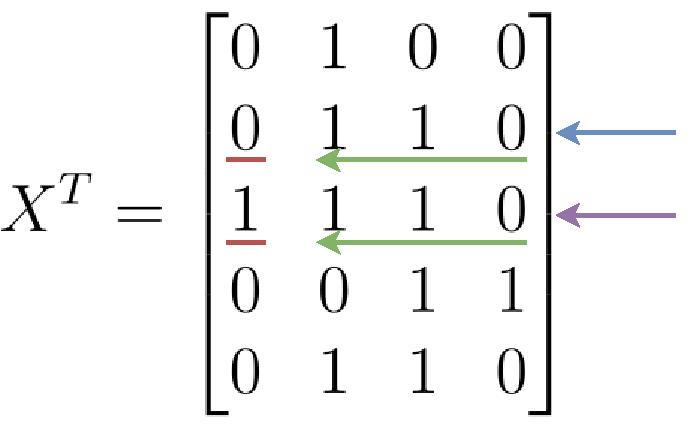
\includegraphics[scale = 0.38]{img/slppanel.pdf}
  \end{figure}
  Si procede quindi salvando la sequenza lineare relativa al pannelli come
  descritto sopra. Si ottiene, con colorati gli stessi risultati della $\LCE$
  query fatta sopra:
  \[0010\,\,{\color{nordgreen}011}{\color{nordred}0}\,\,
    {\color{nordgreen}011}{\color{nordred}1} \,\,1100\,\,0110\]
\end{esempio}
In merito al random access, considerando tale memorizzazione monodimensionale e
invertita, si ha, per accedere alla colonna $k$ della riga $i$-esima del
pannello (con $N$ colonne): 
\begin{equation}
  \label{eq:raslpform}
  x_i[k] = \SLP[N(i+1)-k-1]
\end{equation}
In termini di complessità, si ricorda che, come per il random access,
il calcolo delle $\LCE$ query con $\SLP$ è in tempo proporzionale a: 
\begin{equation}
  \label{eq:timelce}
  \mathcal{O}(\log (\mathit{NM}))
\end{equation}